\documentclass[a4paper]{standalone}
\usepackage{amsmath}
\usepackage{circuitikz}
\usetikzlibrary{fit, shapes, arrows, patterns, decorations.text, decorations.markings}

\begin{document}
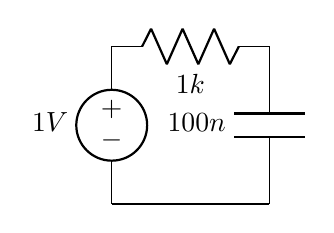
\begin{tikzpicture}[scale=1.00, transform shape, /tikz/circuitikz/bipoles/length=1.50cm, american currents, american voltages, voltage dir=RP]
  \coordinate (1) at (0,2);
  \coordinate (0) at (0,0);
  \coordinate (2) at (2,2);
  \coordinate (0_1) at (2,0);
  \draw (0) to [V, l^=${1V}$, n=V1] (1);
  \draw (1) to [R, l_=${1k}$, n=R1] (2);
  \draw (2) to [C, l_=${100n}$, n=C1] (0_1);
  \draw (0) to (0_1);
\end{tikzpicture}
\end{document}